\documentclass{article}
\usepackage{graphicx}
	\setkeys{Gin}{width=1.0\textwidth}
\usepackage[a4paper]{geometry}
\usepackage{hyperref}
\usepackage{xcolor}
\usepackage{amsmath}
\definecolor{sexygray}{HTML}{1F1F1F}
\begin{document}
	\title{CS 180 MP 3: Naive Bayes}
	\author{Marc Teves\\ 2015-08007\\ THR}
	\maketitle


	Requirements:
	\begin{itemize}
		\item Python 3
		\item \texttt{stemming} python module
		\item \texttt{scikit-learn} module
		\item \texttt{bash} or your favorite shell
	\end{itemize}

	Just run \texttt{main.sh} to start from the very beginning, or run
	\texttt{classify.sh} to classify based on the pre-computed feature vectors.

	\begin{enumerate}
		\item 
			The Bernoulli Naive Bayes achieved a performance measure of 
			around $0.9514$. Refer to Figure 1.
		\item 
			The Multinomial Naive Bayes achieved a performance measure of 
			around $0.9652$. Refer to Figure 1.
		\item 
			Refer to Figure 2. As the lambda smoothing increased, 
			the accuracy decreased along with it.
		\item
			By removing common stop words and words that have less than 3
			characters, the accuracy went up marginally for Bernoulli but went
			down marginally for Multinomial. Refer to Figure 3.
		\item 
			By making the dictionary smaller after reducing it to only stem
			words, accuracy worsened marginally for Bernoulli while it
			increased marginally for Multinomial. Refer to Figure 4.
	\end{enumerate}
	\begin{figure}[h]
		\centering
		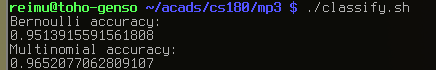
\includegraphics{regular.png}
		\caption{Accuracy for regular dictionary extracted from the training
		set}
	\end{figure}
	\begin{figure}[h]
		\centering
		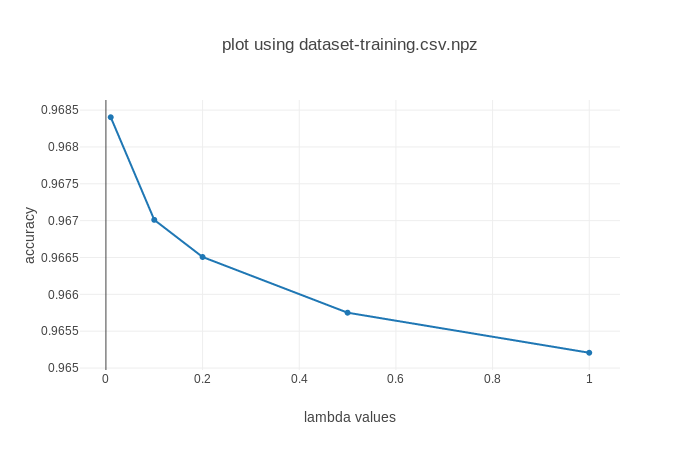
\includegraphics{newplot.png}
		\caption{Plot of accuracy vs. lambda values. Accuracy decreases 
		exponentially slower with higher lambda values.}
	\end{figure}
	\begin{figure}[h]
		\centering
		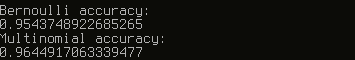
\includegraphics{nostop.png}
		\caption{Accuracy for regular dictionary extracted from the training
		set, with stop words and very small words removed}
	\end{figure}
	\begin{figure}[h]
		\centering
		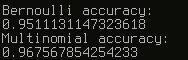
\includegraphics{stem.png}
		\caption{Accuracy for regular dictionary extracted from the training
		set, reduced to only stem words}
	\end{figure}
\end{document}
